\documentclass[12pt]{article}
\title{Assignment 1: CS 754, Advanced Image Processing}
\author{\textbf{Question 6}}
\date{}
\usepackage{amsmath}
\usepackage{amssymb}
\usepackage{hyperref}
\usepackage{ulem}
\usepackage{enumitem}
\usepackage{float}
\usepackage{graphicx}
\usepackage{subcaption}
\usepackage{bm}


\usepackage[margin=0.5in]{geometry}
\begin{document}
\maketitle

\begin{itemize}
    \item In class, we studied a video compressive sensing architecture from the paper `Video from a single exposure coded snapshot' published in ICCV 2011 (See \url{http://www.cs.columbia.edu/CAVE/projects/single_shot_video/}). Such a video camera acquires a `coded snapshot' $E_u$ in a single exposure time interval $u$. This coded snapshot is the superposition of the form $E_u = \sum_{t=1}^T C_t \cdot F_t$ where $F_t$ is the image of the scene at instant $t$ within the interval $u$ and $C_t$ is a randomly generated binary code at that time instant, which modulates $F_t$. Note that $E_u$, $F_t$ and $C_t$ are all 2D arrays. Also, the binary code generation as well as the final summation all occur within the hardware of the camera. Your task here is as follows:
\begin{enumerate}
\item Read the `cars' video in the homework folder in MATLAB using the `mmread' function which has been provided in the homework folder and convert it to grayscale. Extract the first $T = 3$ frames of the video.
\item Generate a $H \times W \times T$ random code pattern whose elements lie in $\{0,1\}$. Compute a coded snapshot using the formula mentioned and add zero mean Gaussian random noise of standard deviation 2 to it. Display the coded snapshot in your report.
\item Given the coded snapshot and assuming full knowledge of $C_t$ for all $t$ from 1 to $T$, your task is to estimate the original video sequence $F_t$. For this you should rewrite the aforementioned equation in the form $\boldsymbol{Ax} = \boldsymbol{b}$ where $\boldsymbol{x}$ is an unknown vector (vectorized form of the video sequence). Mention clearly what $\boldsymbol{A}$ and $\boldsymbol{b}$ are, in your report.
\item You should perform the reconstruction using Orthogonal Matching Pursuit (OMP). For computational efficiency, we will do this reconstruction patchwise. Write an equation of the form $\boldsymbol{Ax} = \boldsymbol{b}$ where $\boldsymbol{x}$ represents the $i^{th}$ patch from the video and having size (say) $8 \times 8 \times T$ and mention in your report what $\boldsymbol{A}$ and $\boldsymbol{b}$ stand for. For perform the reconstruction, assume that each $8 \times 8$ slice in the patch is sparse or compressible in the 2D-DCT basis. Carefully work out the error term in the OMP algorithm, and explain this in your report!
\item Repeat the reconstruction for all overlapping patches and average across the overlapping pixels to yield the final reconstruction. Display the reconstruction and mention the relative mean squared error between reconstructed and original Data:, in your report as well as in the code. 
\item Repeat this exercise for $T = 5, T = 7$ and mention the mention the relative mean squared error between reconstructed and original Data: again.
\item \textbf{Note: To save time, extract a portion of about $120 \times 240$ around the lowermost car in the cars video and work entirely with it. In fact, you can show all your results just on this part. Some sample results are included in the homework folder.}
\item Repeat the experiment with any consecutive 5 frames of the `flame' video from the homework folder.
\end{enumerate}
\vspace*{0.5cm}\\
\textbf{Answer:} \\
\begin{enumerate}
    \item The first T = 3 frames of the given 'cars.avi' video resized to $120 \times 240$ around the lowermost car are shown below
    
    \begin{figure}[H]
        \centering
        \begin{minipage}{.45\textwidth}
            \centering
            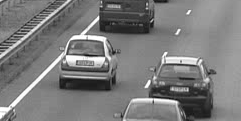
\includegraphics[width=\linewidth]{results/cars_3_orig_1.png}
            \caption*{Frame 1}
        \end{minipage}
        \begin{minipage}{.45\textwidth}
            \centering
            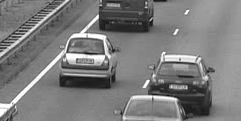
\includegraphics[width=\linewidth]{results/cars_3_orig_2.png}
            \caption*{Frame 2}
        \end{minipage}
        \begin{minipage}{.45\textwidth}
            \centering
            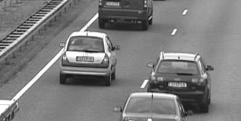
\includegraphics[width=\linewidth]{results/cars_3_orig_3.png}
            \caption*{Frame 3}
        \end{minipage}
    \end{figure}
    

    \item The coded snapshot computed using the equation $E_u = \sum_{t=1}^3 C_t \cdot F_t$ (where $F_t$ is the frame at time T, $C_t$ is the code at time T) is shown below.
    \begin{figure}[H]
        \centering
        \begin{minipage}{.45\textwidth}
            \centering
            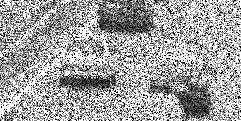
\includegraphics[width=\linewidth]{results/cars_noisy_snapshot_3.png}
            \caption*{Coded snapshot}
        \end{minipage}
    \end{figure}

    \item The coded snapshot is computed using the following equation,
    \begin{equation}
        E_u = \sum_{t=1}^T C_t \cdot F_t
    \end{equation}
    where $F_t$ is the frame at time t, $C_t$ is the binary code at time t. In our case the frames $F_t$ is the original signal and the coded snapshot is the compressed measurement. We have to represent the above equation in the form $y = A x$
    We can do so by vectorizing the signals. \\
    To vectorize $F_t$ we can convert video frame to a vector by stacking columns one the other. All the video frames upto time T are then stacked one below the other to form a single column vector. Hence,
    \begin{gather*}
        x = \text{Vectorized video frames} \in \mathbb{R}^{HWT \times 1}
    \end{gather*} 
    The compressed measurement can be considered to be the vectorized version of the coded snapshot. This is obtained by stacking columns one the coded snapshot to form a single column vector. Hence,
    \begin{gather*}
        y = \text{Vectorized coded snapshot} \in \mathbb{R}^{HW \times 1}
    \end{gather*}
    We can consider the matrix A to be of the form,
    \begin{gather*}
        A = [ \ diag(C_1 (:)) \ | \ diag(C_2 (:)) \ | \ ... \ | \ diag(C_T (:)) ] \in \mathbb{R}^{HW \times HWT}
    \end{gather*}
    i.e. we first stack the columns of the matrix $C_t$ to form a single vector, then construct a diagonal matrix with the diagonal entries as the vectorized version of the code $C_t$. Finally we stack the columns of the diagonal matrix formed from $ C_{t} \forall t$ to form the matrix $A$.

    \item In this problem we have added noise ($\eta$) from Gaussian distribution with $\sigma = 2$. Hence, with high proability the magnitude of $\eta$ will lie within 3 standard deviations from the mean. Hence, the error term in the OMP algorithm is can be set to be greater than $9m\sigma^2$ i.e.,
    $$ \epsilon \geq 9m\sigma^2 $$
    where $m$ is the number of measurements. Since, we are performing the reconstruction on $8 \times 8$ patches, we can assume that the number of measurements m are 64. Also, in the code we have converted the image pixel to range of 0 to 1. Hence, the sigma value should be modified to be $2/255$ to account for the range of pixel values. Hence, the lower bound on epsilon should be set to,
    \begin{gather*}
        \begin{aligned}
            \epsilon &\geq 9m\sigma^2 \\
            &\geq 9*64*2/(255^2) = 0.0354
        \end{aligned}
    \end{gather*}

    In the code we have set $\epsilon$ to be 0.1 to reduce the computational time for the reconstruction.

    \item For T= 3, the RMSE between the original Data: and the reconstructed Data: is \textbf{0.0114}. \\
    The reconstructed video frames along with the original video frames are shown below.

    \begin{figure}[H]
        \centering
        \begin{minipage}{.45\textwidth}
            \centering
            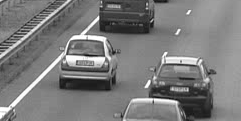
\includegraphics[width=\linewidth]{results/cars_3_orig_1.png}
            \caption*{Original Data: frame 1}
        \end{minipage}
        \begin{minipage}{.45\textwidth}
            \centering
            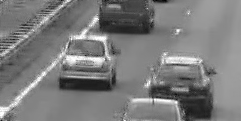
\includegraphics[width=\linewidth]{results/cars_3_recon_1.png}
            \caption*{Reconstructed Data: frame 1}
        \end{minipage}
    \end{figure}

    \begin{figure}[H]
        \centering
        \begin{minipage}{.45\textwidth}
            \centering
            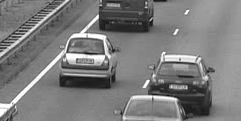
\includegraphics[width=\linewidth]{results/cars_3_orig_2.png}
            \caption*{Original Data: frame 2}
        \end{minipage}
        \begin{minipage}{.45\textwidth}
            \centering
            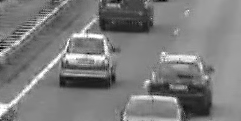
\includegraphics[width=\linewidth]{results/cars_3_recon_2.png}
            \caption*{Reconstructed Data: frame 2}
        \end{minipage}
    \end{figure}

    \begin{figure}[H]
        \centering
        \begin{minipage}{.45\textwidth}
            \centering
            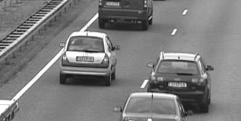
\includegraphics[width=\linewidth]{results/cars_3_orig_3.png}
            \caption*{Original Data: frame 3}
        \end{minipage}
        \begin{minipage}{.45\textwidth}
            \centering
            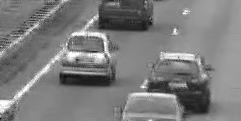
\includegraphics[width=\linewidth]{results/cars_3_recon_3.png}
            \caption*{Reconstructed Data: frame 3}
        \end{minipage}
    \end{figure}

    \item \textbf{For T = 5} \\
    The coded snapshot of the video for T= 5 is as follows
    \begin{figure}[H]
        \centering
        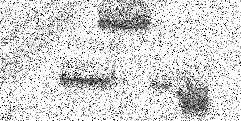
\includegraphics[width=0.5\linewidth]{results/cars_noisy_snapshot_5.png}
        \caption*{Coded snapshot for T = 5}
    \end{figure}

    The RMSE between the original Data: and the reconstructed Data: is \textbf{0.0193}. \\
    The reconstructed video frames along with the original video frames are shown below.
    
    
    
    \begin{figure}[H]
        \centering
        \begin{minipage}{.45\textwidth}
            \centering
            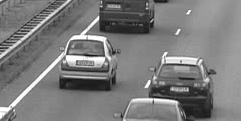
\includegraphics[width=\linewidth]{results/cars_5_orig_1.png}
            \caption*{Original Data: frame 1}
        \end{minipage}
        \begin{minipage}{.45\textwidth}
            \centering
            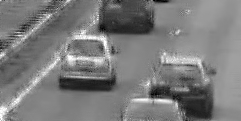
\includegraphics[width=\linewidth]{results/cars_5_recon_1.png}
            \caption*{Reconstructed Data: frame 1}
        \end{minipage}
    \end{figure}
    
    \begin{figure}[H]
        \centering
        \begin{minipage}{.45\textwidth}
            \centering
            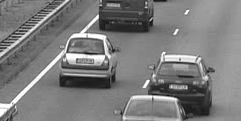
\includegraphics[width=\linewidth]{results/cars_5_orig_2.png}
            \caption*{Original Data: frame 2}
        \end{minipage}
        \begin{minipage}{.45\textwidth}
            \centering
            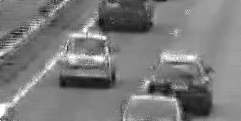
\includegraphics[width=\linewidth]{results/cars_5_recon_2.png}
            \caption*{Reconstructed Data: frame 2}
        \end{minipage}
    \end{figure}
    
    \begin{figure}[H]
        \centering
        \begin{minipage}{.45\textwidth}
            \centering
            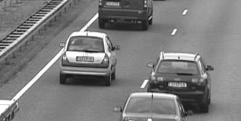
\includegraphics[width=\linewidth]{results/cars_5_orig_3.png}
            \caption*{Original Data: frame 3}
        \end{minipage}
        \begin{minipage}{.45\textwidth}
            \centering
            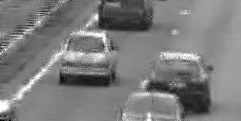
\includegraphics[width=\linewidth]{results/cars_5_recon_3.png}
            \caption*{Reconstructed Data: frame 3}
        \end{minipage}
    \end{figure}
    
    \begin{figure}[H]
        \centering
        \begin{minipage}{.45\textwidth}
            \centering
            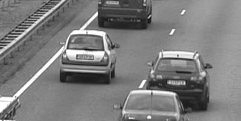
\includegraphics[width=\linewidth]{results/cars_5_orig_4.png}
            \caption*{Original Data: frame 4}
        \end{minipage}
        \begin{minipage}{.45\textwidth}
            \centering
            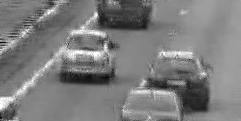
\includegraphics[width=\linewidth]{results/cars_5_recon_4.png}
            \caption*{Reconstructed Data: frame 4}
        \end{minipage}
    \end{figure}


    \begin{figure}[H]
        \centering
        \begin{minipage}{.45\textwidth}
            \centering
            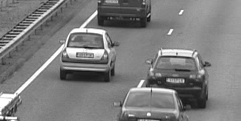
\includegraphics[width=\linewidth]{results/cars_5_orig_5.png}
            \caption*{Original Data: frame 5}
        \end{minipage}
        \begin{minipage}{.45\textwidth}
            \centering
            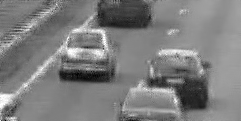
\includegraphics[width=\linewidth]{results/cars_5_recon_5.png}
            \caption*{Reconstructed Data: frame 5}
        \end{minipage}
    \end{figure}
    
    \\
    \textbf{For T = 7} \\
    The coded snapshot of the video for T= 7 is as follows
    \begin{figure}[H]
        \centering
        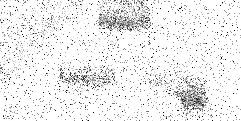
\includegraphics[width=0.5\linewidth]{results/cars_noisy_snapshot_7.png}
        \caption*{Coded snapshot for T = 7}
    \end{figure}

    The RMSE between the original Data: and the reconstructed Data: is \textbf{0.0301}. \\

    The reconstructed video frames along with the original video frames are shown below.

    \begin{figure}[H]
        \centering
        \begin{minipage}{.45\textwidth}
            \centering
            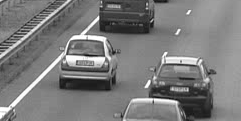
\includegraphics[width=\linewidth]{results/cars_7_orig_1.png}
            \caption*{Original Data: frame 1}
        \end{minipage}
        \begin{minipage}{.45\textwidth}
            \centering
            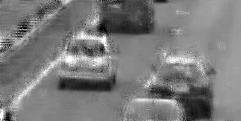
\includegraphics[width=\linewidth]{results/cars_7_recon_1.png}
            \caption*{Reconstructed Data: frame 1}
        \end{minipage}
    \end{figure}

    \begin{figure}[H]
        \centering
        \begin{minipage}{.45\textwidth}
            \centering
            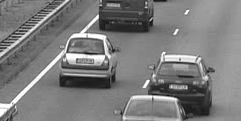
\includegraphics[width=\linewidth]{results/cars_7_orig_2.png}
            \caption*{Original Data: frame 2}
        \end{minipage}
        \begin{minipage}{.45\textwidth}
            \centering
            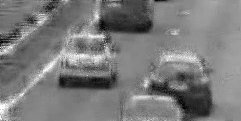
\includegraphics[width=\linewidth]{results/cars_7_recon_2.png}
            \caption*{Reconstructed Data: frame 2}
        \end{minipage}
    \end{figure}

    \begin{figure}[H]
        \centering
        \begin{minipage}{.45\textwidth}
            \centering
            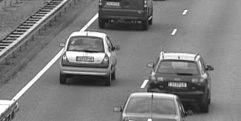
\includegraphics[width=\linewidth]{results/cars_7_orig_3.png}
            \caption*{Original Data: frame 3}
        \end{minipage}
        \begin{minipage}{.45\textwidth}
            \centering
            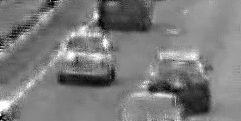
\includegraphics[width=\linewidth]{results/cars_7_recon_3.png}
            \caption*{Reconstructed Data: frame 3}
        \end{minipage}
    \end{figure}

    \begin{figure}[H]
        \centering
        \begin{minipage}{.45\textwidth}
            \centering
            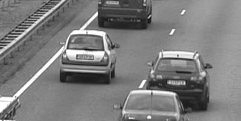
\includegraphics[width=\linewidth]{results/cars_7_orig_4.png}
            \caption*{Original Data: frame 4}
        \end{minipage}
        \begin{minipage}{.45\textwidth}
            \centering
            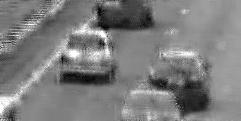
\includegraphics[width=\linewidth]{results/cars_7_recon_4.png}
            \caption*{Reconstructed Data: frame 4}
        \end{minipage}
    \end{figure}
    
    \begin{figure}[H]
        \centering
        \begin{minipage}{.45\textwidth}
            \centering
            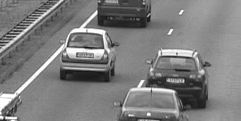
\includegraphics[width=\linewidth]{results/cars_7_orig_5.png}
            \caption*{Original Data: frame 5}
        \end{minipage}
        \begin{minipage}{.45\textwidth}
            \centering
            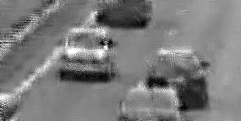
\includegraphics[width=\linewidth]{results/cars_7_recon_5.png}
            \caption*{Reconstructed Data: frame 5}
        \end{minipage}
    \end{figure}

    \begin{figure}[H]
        \centering
        \begin{minipage}{.45\textwidth}
            \centering
            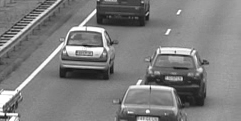
\includegraphics[width=\linewidth]{results/cars_7_orig_6.png}
            \caption*{Original Data: frame 6}
        \end{minipage}
        \begin{minipage}{.45\textwidth}
            \centering
            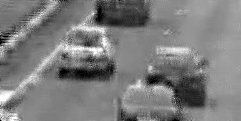
\includegraphics[width=\linewidth]{results/cars_7_recon_6.png}
            \caption*{Reconstructed Data: frame 6}
        \end{minipage}
    \end{figure}

    \begin{figure}[H]
        \centering
        \begin{minipage}{.45\textwidth}
            \centering
            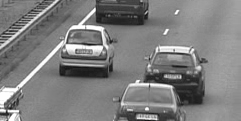
\includegraphics[width=\linewidth]{results/cars_7_orig_7.png}
            \caption*{Original Data: frame 7}
        \end{minipage}
        \begin{minipage}{.45\textwidth}
            \centering
            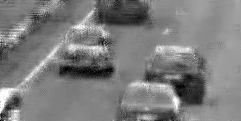
\includegraphics[width=\linewidth]{results/cars_7_recon_7.png}
            \caption*{Reconstructed Data: frame 7}
        \end{minipage}
    \end{figure}

    \item For the results on the 'cars.avi' video we have only considered the lower $120 \times 240$ pixels of the video.
    \item \textbf{Results for the Flame Video}
    Note: We have considered the first 5 frames of the video. Also for this part we have considered the entire image frame for the reconstruction.
    The coded snapshot of the video for T= 5 is as follows
    \begin{figure}[H]
        \centering
        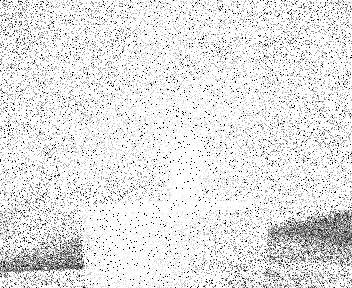
\includegraphics[width=0.5\linewidth]{results/flame_noisy_snapshot_5.png}
        \caption*{Coded snapshot for T = 5}
    \end{figure}

    The RMSE between the original Data: and the reconstructed Data: is \textbf{0.0011}. \\

    The reconstructed video frames along with the original video frames are shown below.
    \begin{figure}[H]
        \centering
        \begin{minipage}{.45\textwidth}
            \centering
            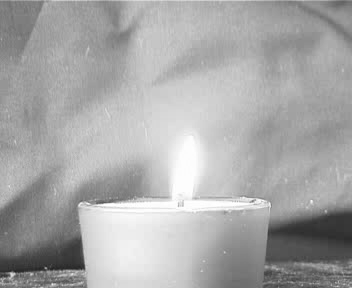
\includegraphics[width=\linewidth]{results/flame_5_orig_1.png}
            \caption*{Original Data: frame 1}
        \end{minipage}
        \begin{minipage}{.45\textwidth}
            \centering
            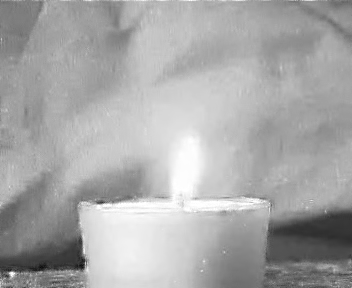
\includegraphics[width=\linewidth]{results/flame_5_recon_1.png}
            \caption*{Reconstructed Data: frame 1}
        \end{minipage}
    \end{figure}

    \begin{figure}[H]
        \centering
        \begin{minipage}{.45\textwidth}
            \centering
            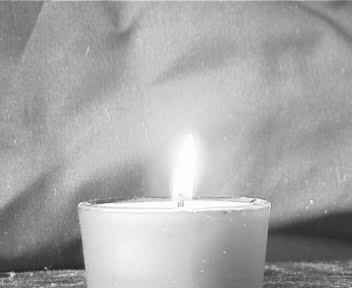
\includegraphics[width=\linewidth]{results/flame_5_orig_2.png}
            \caption*{Original Data: frame 2}
        \end{minipage}
        \begin{minipage}{.45\textwidth}
            \centering
            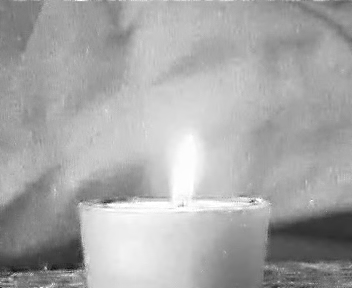
\includegraphics[width=\linewidth]{results/flame_5_recon_2.png}
            \caption*{Reconstructed Data: frame 2}
        \end{minipage}
    \end{figure}

    \begin{figure}[H]
        \centering
        \begin{minipage}{.45\textwidth}
            \centering
            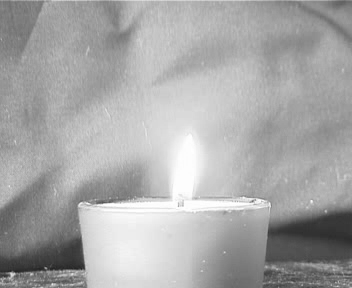
\includegraphics[width=\linewidth]{results/flame_5_orig_3.png}
            \caption*{Original Data: frame 3}
        \end{minipage}
        \begin{minipage}{.45\textwidth}
            \centering
            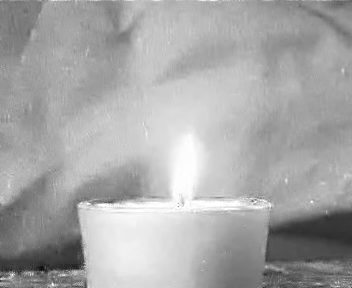
\includegraphics[width=\linewidth]{results/flame_5_recon_3.png}
            \caption*{Reconstructed Data: frame 3}
        \end{minipage}
    \end{figure}

    \begin{figure}[H]
        \centering
        \begin{minipage}{.45\textwidth}
            \centering
            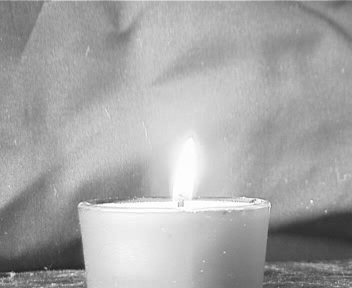
\includegraphics[width=\linewidth]{results/flame_5_orig_4.png}
            \caption*{Original Data: frame 4}
        \end{minipage}
        \begin{minipage}{.45\textwidth}
            \centering
            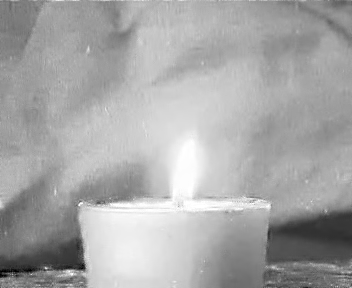
\includegraphics[width=\linewidth]{results/flame_5_recon_4.png}
            \caption*{Reconstructed Data: frame 4}
        \end{minipage}
    \end{figure}

    \begin{figure}[H]
        \centering
        \begin{minipage}{.45\textwidth}
            \centering
            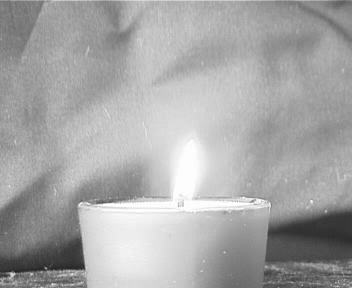
\includegraphics[width=\linewidth]{results/flame_5_orig_5.png}
            \caption*{Original Data: frame 5}
        \end{minipage}
        \begin{minipage}{.45\textwidth}
            \centering
            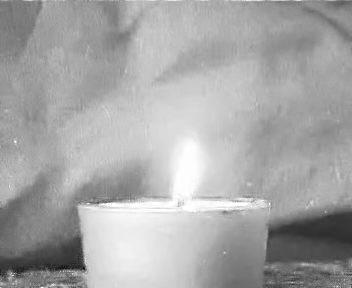
\includegraphics[width=\linewidth]{results/flame_5_recon_5.png}
            \caption*{Reconstructed Data: frame 5}
        \end{minipage}
    \end{figure}

\end{enumerate}


\end{itemize}
\end{document}